% !TeX root = ../main.tex

\chapter{文件系统性能测试}
\label{cha:evaluation}

% 实验结果的分析讨论及与理论计算结果的比较

本课题实现的文件系统部署在 3 台配置相同的服务器组成的微型集群上进行测试。测试环境的细节如下:每台服务器搭载 4 个 18 核 Intel\textregistered ~Xeon\textregistered ~Gold 6240M CPU,频率为 2.60 GHz。每台服务器装有 200 GB 内存,以及两个大小为 800GB 的 Intel\textregistered ~Optane\textsuperscript{\texttrademark} DC 持久性内存;3 台服务器上合计 6 个 NVM 设备,用于模拟 6 个不同的存储节点。每台服务器安装有两个带宽为 100Gbps 的 Mellanox InfiniBand 网卡(实验时只使用其中一个),服务器之间通过它们建立 RDMA 网络连接。

测试时,通过一个客户机与上述集群通信,完成各种文件系统操作,并测试其性能。

\section{不同可用性策略的开销}
\label{sec:ch4_avail_cost}

本节测试不同可用性策略的时间开销。在文件系统其它部分不变的情况下,在可用性策略层实现不同的策略,并测试其耗时。

一共测试四种不同的情况:无可用性策略(None)、三副本(Repl)、朴素 Reed-Solomon 码 $RS(4, 2)$(RS),以及 Clay Code 编码(Clay)。每种情况下的时间开销分为两部分:耗费在 RDMA 上的网络通信开销,以及耗费在纠删码编码上的计算开销。的考虑到不同读写粒度可能对可用性策略的开销带来不同影响,分别以 4KB、16KB 和 64KB 作为读写粒度进行测试。由于测试的读写数据量之间相差较大,因此将测得的开销数据向三副本策略归一化。

测试结果如图 ~\ref{fig:avail_cost} 所示:

\begin{figure}[H]
    \centering
    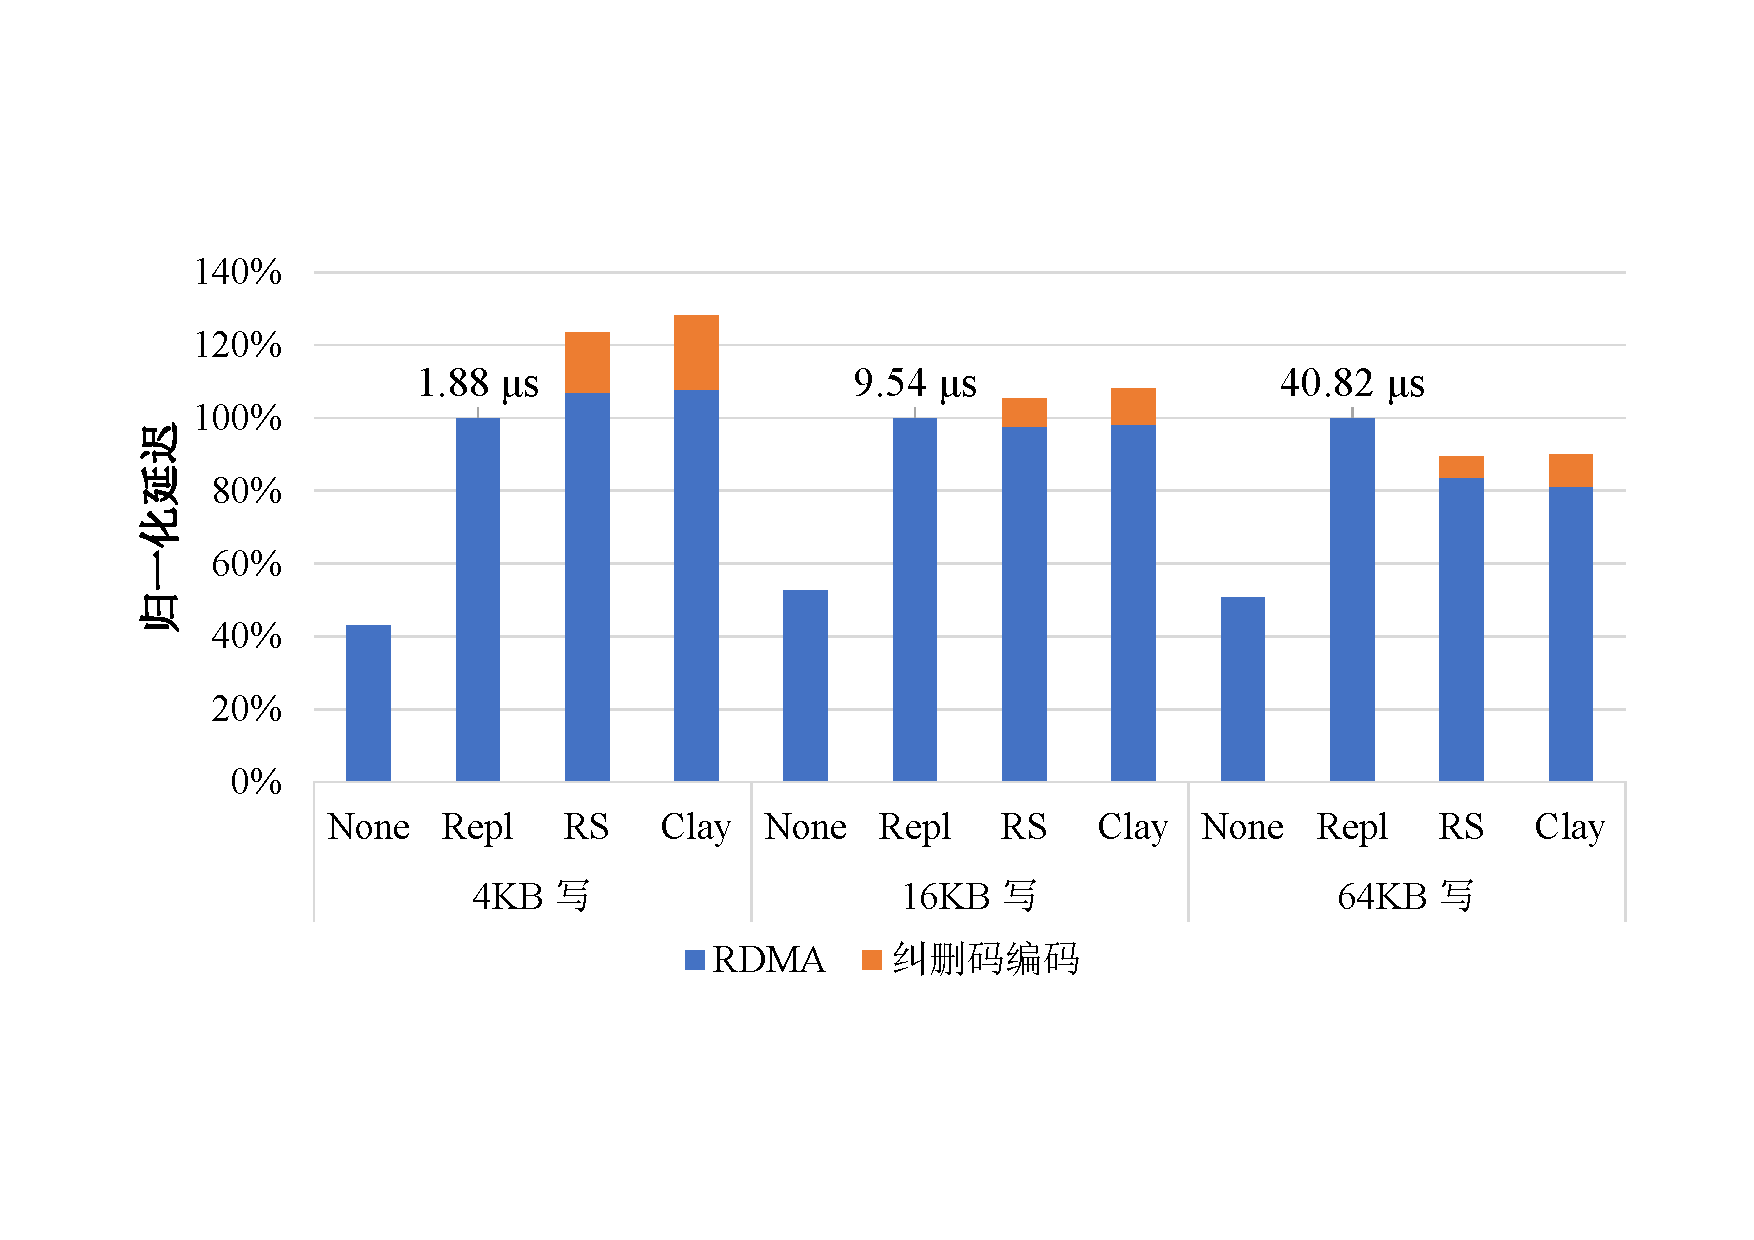
\includegraphics[width=13.5cm]{avail-cost.pdf}
    \caption{不同可用性策略的归一化开销}
    \label{fig:avail_cost}
\end{figure}

可见,虽然纠删码的编码带来了额外的 CPU 计算开销,在 4KB 读写时其延迟高出三副本策略 20\% $\sim$ 40\%;但在读写粒度较大时,其网络通信量较小、并行度高,在 RDMA 通信上节省了较多时间,读写延迟反而更低;以 64KB 为粒度读写时,$RS(4, 2)$ 和 Clay Code 带来的延迟均比三副本策略低 10\% 左右。测试表明,纠删码在文件系统访问粒度较大时有良好的表现;而在访问粒度较小时,相比于传统数据备份策略,纠删码虽然会引入较大比例的额外延迟,但这些延迟的绝对值很小(本例中不超过 $\SI{1}{\us}$),对系统整体性能的影响并不大。

\section{读写带宽和延迟}
\label{sec:ch4_rw_bw_latency}

本节测试文件系统的读写延迟和读写带宽,表征文件系统的整体性能。读写以 4KB 粒度进行。

测得的 4KB 读写操作延迟如表 ~\ref{tab:avail_cost} 所示:

\begin{table}[htb]
    \centering
    \caption[不同可用性策略下的 4KB 读写延迟]{不同可用性策略下的 4KB 读写延迟(单位:$\SI{}{\us}$)}
    \label{tab:avail_cost}
      \begin{tabular}{ccc}
        \toprule[1.5pt]
        {\heiti 可用性策略} & {\heiti 读延迟} & {\heiti 写延迟} \\\midrule[1pt]
        三副本 & 18.92 & 33.46 \\
        Reed-Solomon 编码 & 22.15 & 38.75 \\
        Clay Code 编码 & 22.30 & 40.33 \\
        \bottomrule[1.5pt]
      \end{tabular}
\end{table}

读写延迟由 ~\ref{sec:ch4_avail_cost} 节所述的可用性策略开销,以及文件系统的元数据操作开销共同构成。可以明显看出,元数据操作开销占了总开销的绝大部分。虽然这些开销绝大部分由 LocoFS 引入,针对其进行优化理应能获得更低的读写延迟;但由于这并非主要研究目标,因此本课题并未予以实现。

测得的 4KB 读写操作带宽如下:

\begin{figure}[H]
    \centering
    \subcaptionbox{4KB 写\label{fig:thpt_write}}[13.5cm] 
        {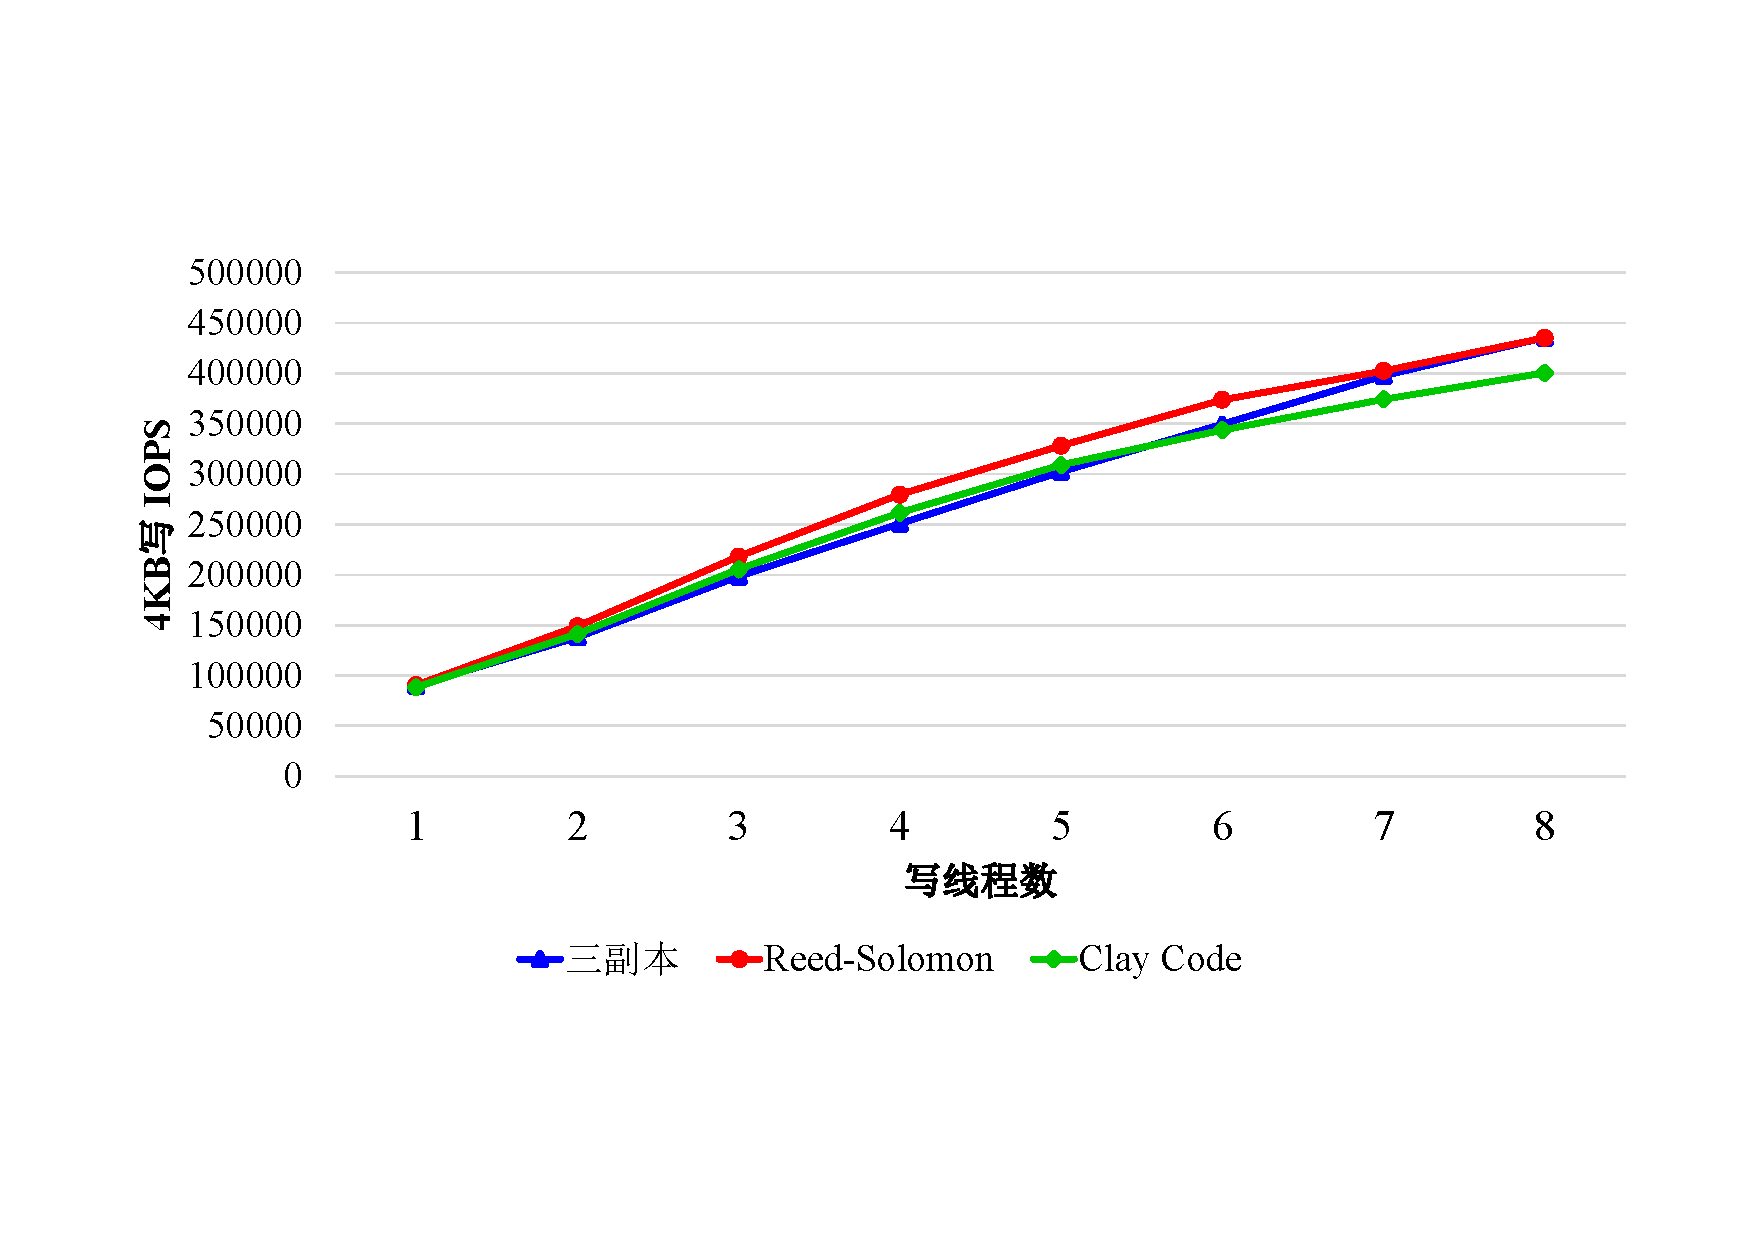
\includegraphics[width=13.5cm]{thpt-write.pdf}}
    \subcaptionbox{4KB 读\label{fig:thpt_read}}[13.5cm] 
        {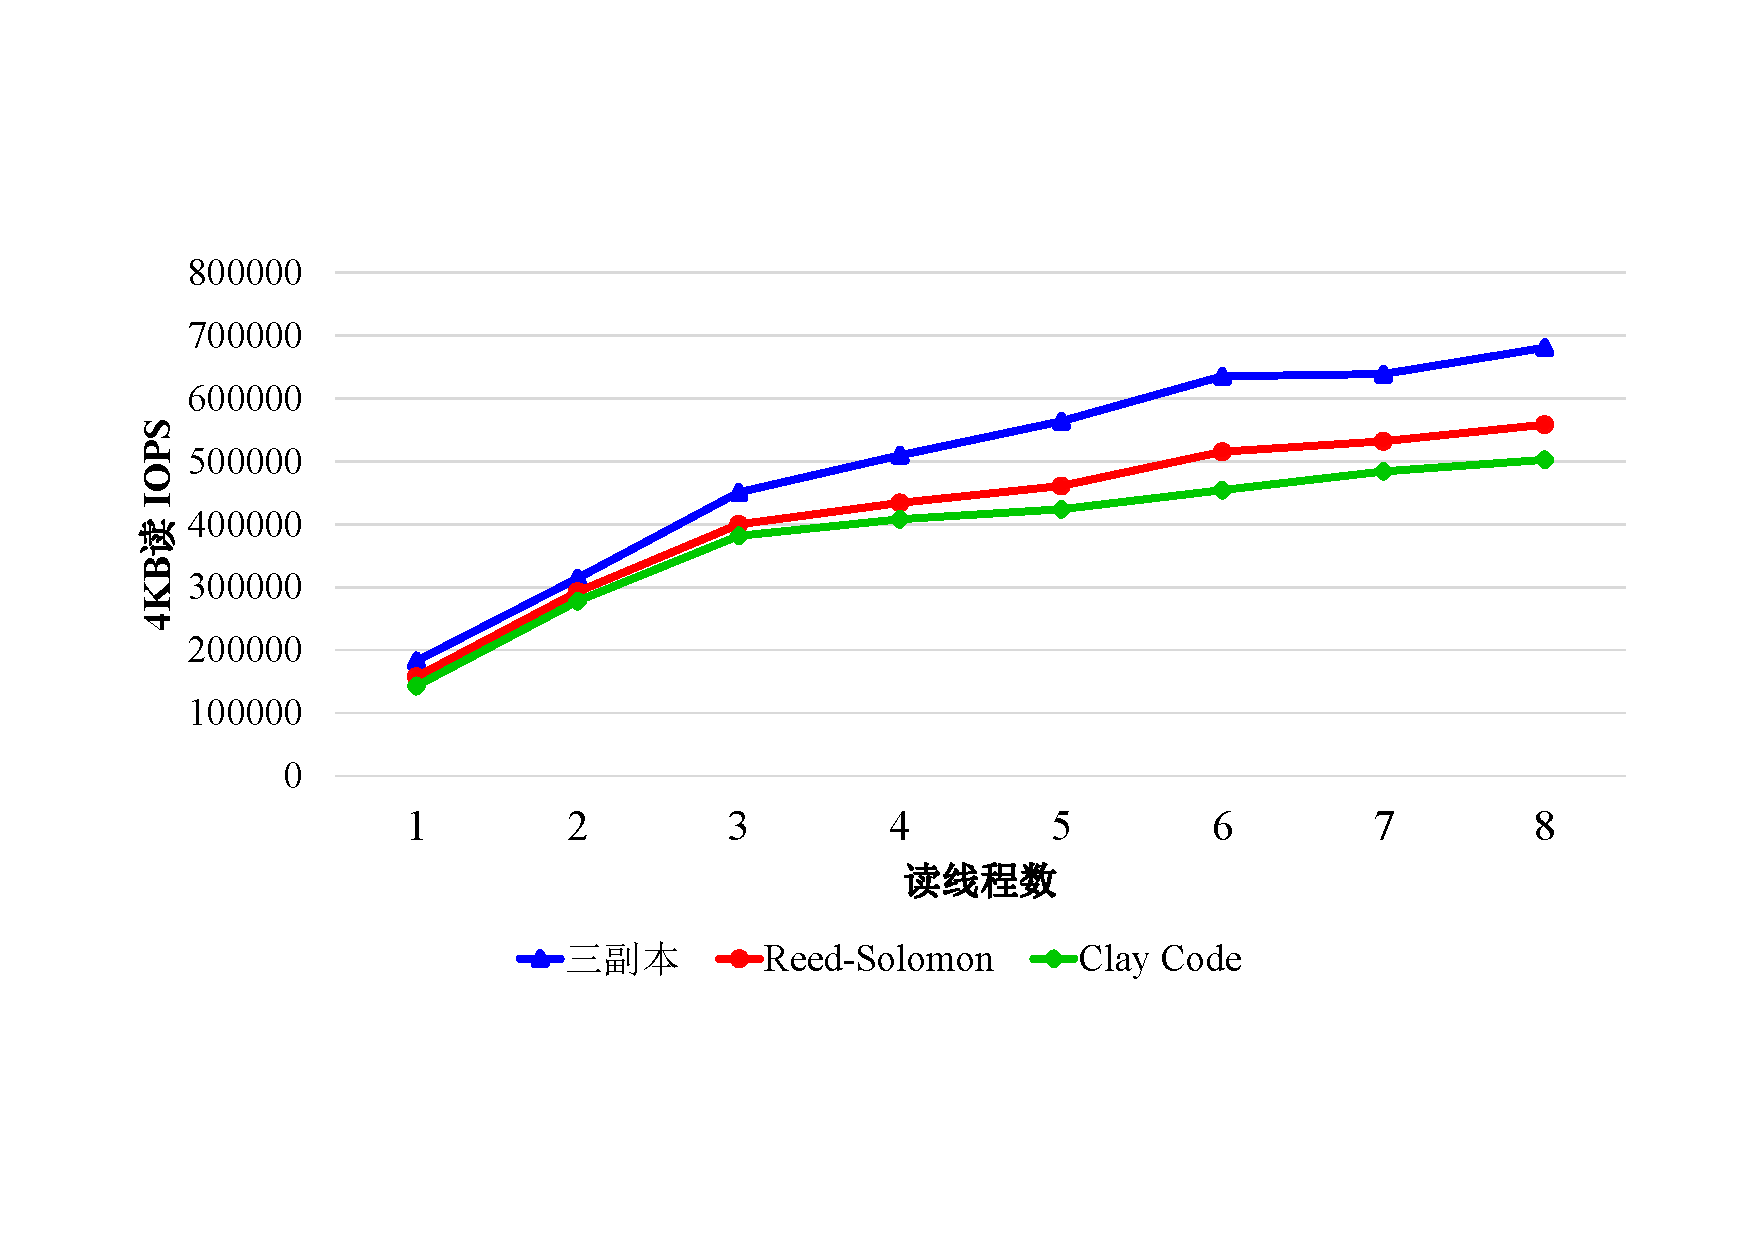
\includegraphics[width=13.5cm]{thpt-read.pdf}}   
    \caption{4KB 读写带宽曲线}
    \label{fig:thpt}
\end{figure}

写数据方面,本课题实现的文件系统在写线程数较少时,其性能表现了良好的线性增长趋势。并且,Reed-Solomon 码的表现略优于三副本策略,写带宽提升最大达到 11\%。这是由于其写入的数据量相较于三副本策略少 50\%,节省了 RDMA 带宽,因此取得了较好的表现。在使用 Clay Code 编码时,系统的写带宽相对较低,相比三副本而言最多降低了 8\%。考虑到纠删码策略相比于三副本节省了 50\% 的 NVM 存储空间,这一性能下降是完全可以接受的。

读数据方面,本课题实现的文件系统在读线程数少于 3 时表现良好的性能线性增长,但在并发数继续增加后性能增长进入瓶颈。相较于三副本策略,使用 Reed-Solomon 码时,系统的读带宽降低了 6\% $\sim$ 18\%;使用 Clay Code 编码时,系统的写带宽降低了 11\% $\sim$ 30\%。三副本策略在读数据时表现更好,是因为它没有纠删码解码开销;并且,虽然其读取的数据量与纠删码策略相同,但只需从一个节点读取一次;而纠删码需要从多个节点各读取一次,引入了额外的网络通信开销。

\section{文件系统可用性及稳定性}
\label{sec:ch4_avail_test}

在第 ~\ref{cha:design} 章中,我们从理论上论证了本课题中的文件系统能提供一定的可用性保障:\ref{sec:ch3_avail} 节证明了该系统能容忍部分节点故障,\ref{subsec:ch3_first_k} 节证明了该系统能容忍部分节点访问延迟的突然升高。本节针对上述两点进行测试,证明文件系统具备预想的可用性等级。

\subsection{纠删码策略的可用性}
\label{subsec:ch4_fail_test}

本小节测试文件系统在节点失效时的工作状况。客户端连续进行约 60 秒的 4KB 文件读写;在进行到约 24 秒时,手动结束一个节点上的文件系统进程。由于一台服务器使用 2 个 NVM 设备模拟 2 个远程节点,因此这相当于模拟两个节点同时发生故障,达到了系统的最大容错能力。合计测得约 273.1 万次读写的延迟数据,经过均匀采样后,绘制曲线如下:

\begin{figure}[H]
    \centering
    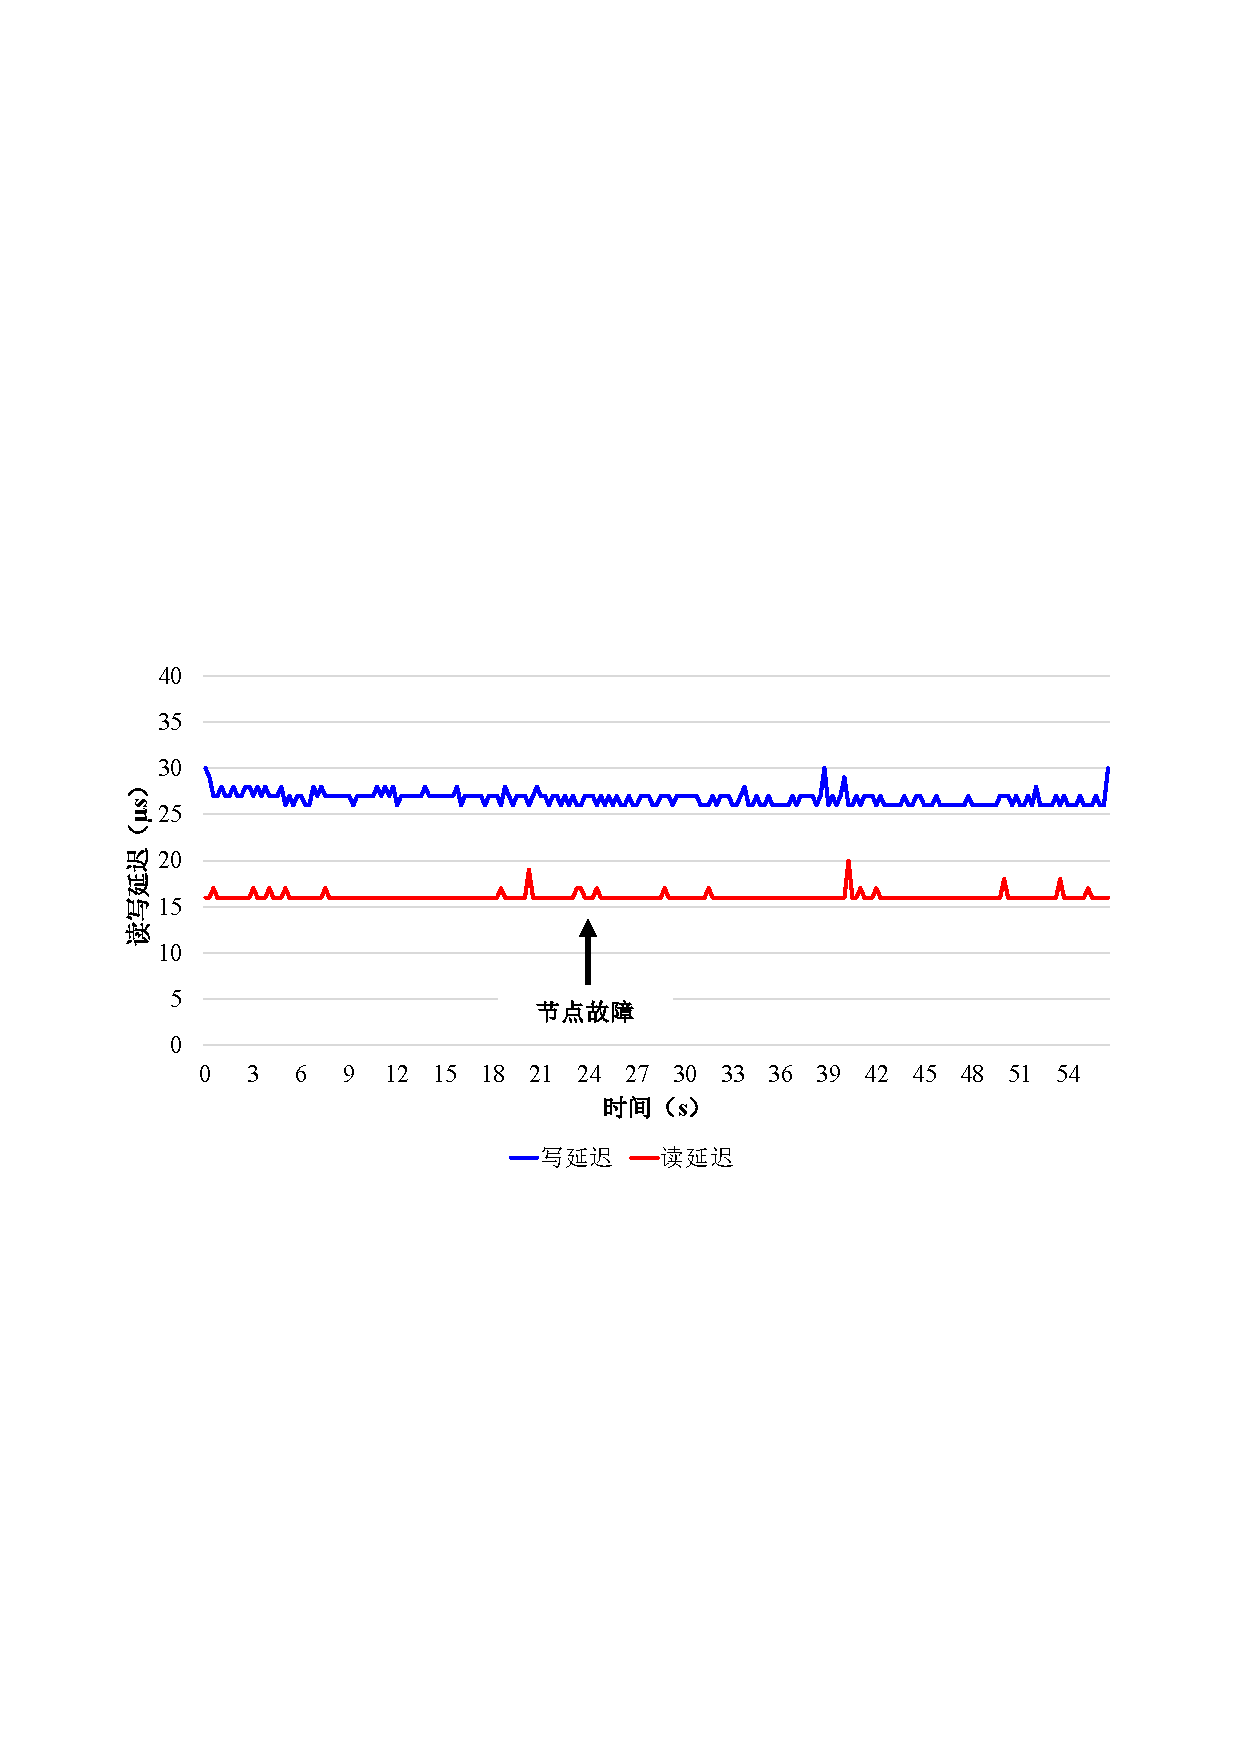
\includegraphics[width=13.5cm]{avail-fail.pdf}
    \caption{节点故障前后的 4KB 读写延迟曲线}
    \label{fig:avail_fail}
\end{figure}

可见,在节点故障前后,系统的读写延迟没有明显改变,客户端仍然能正常执行文件系统操作。这表明系统的容错能力符合预期。

\subsection{前-k 读取策略对读取性能稳定性的影响}
\label{subsec:ch4_first_k_test}

本小节测试前-k 读取策略对读操作性能稳定性的影响。客户端进行两次约 20 秒的 4KB 文件读取,其中一次使用前-k 读取策略,另一次不使用该策略,而是随机选择恰好 $k$ 个节点读取数据,作对照组。每次均测得约 112.0 万次读取延迟数据,绘制曲线如下:

\begin{figure}[H]
    \centering
    \subcaptionbox{禁用前-k 读取\label{fig:no_first_k}}[13.5cm] 
        {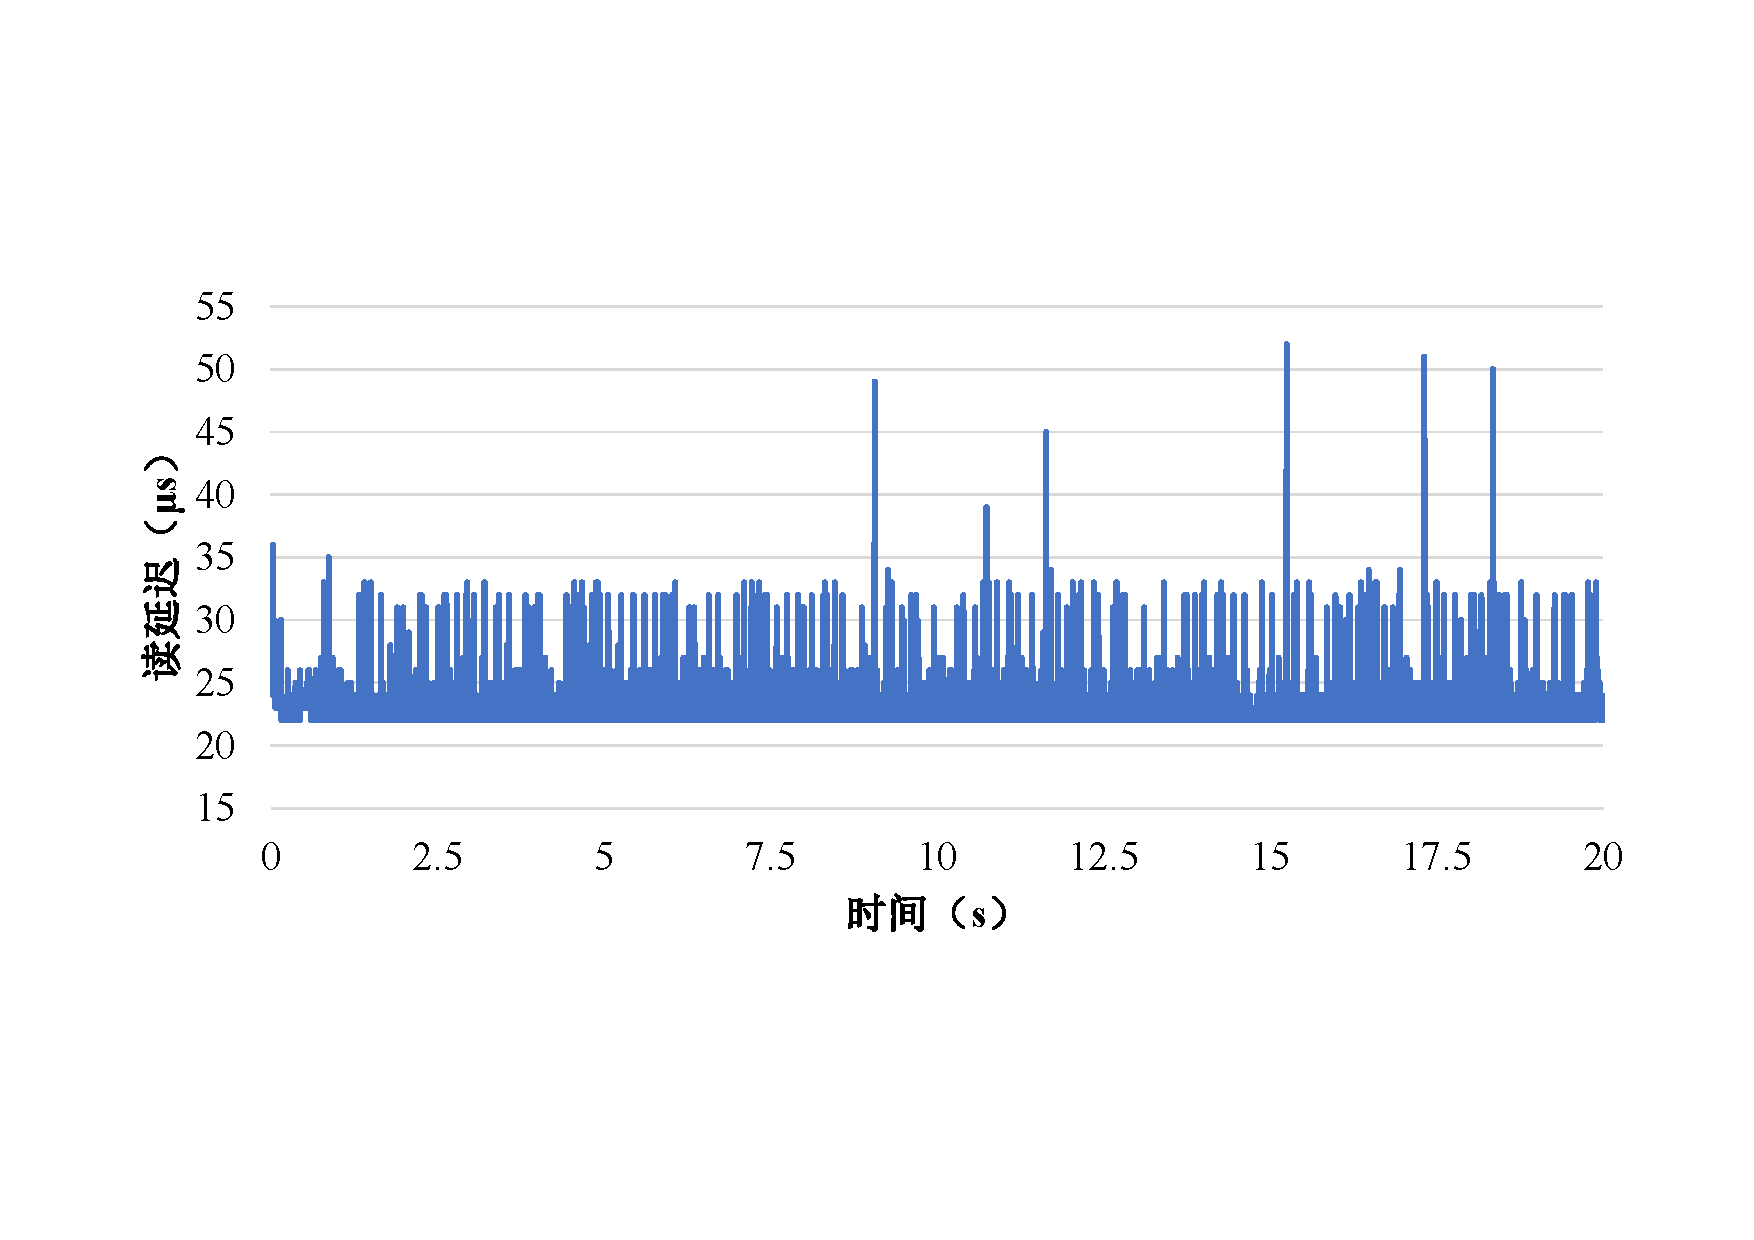
\includegraphics[width=13.5cm]{no-firstk.pdf}}
    \subcaptionbox{使用前-k 读取\label{fig:with_first_k}}[13.5cm] 
        {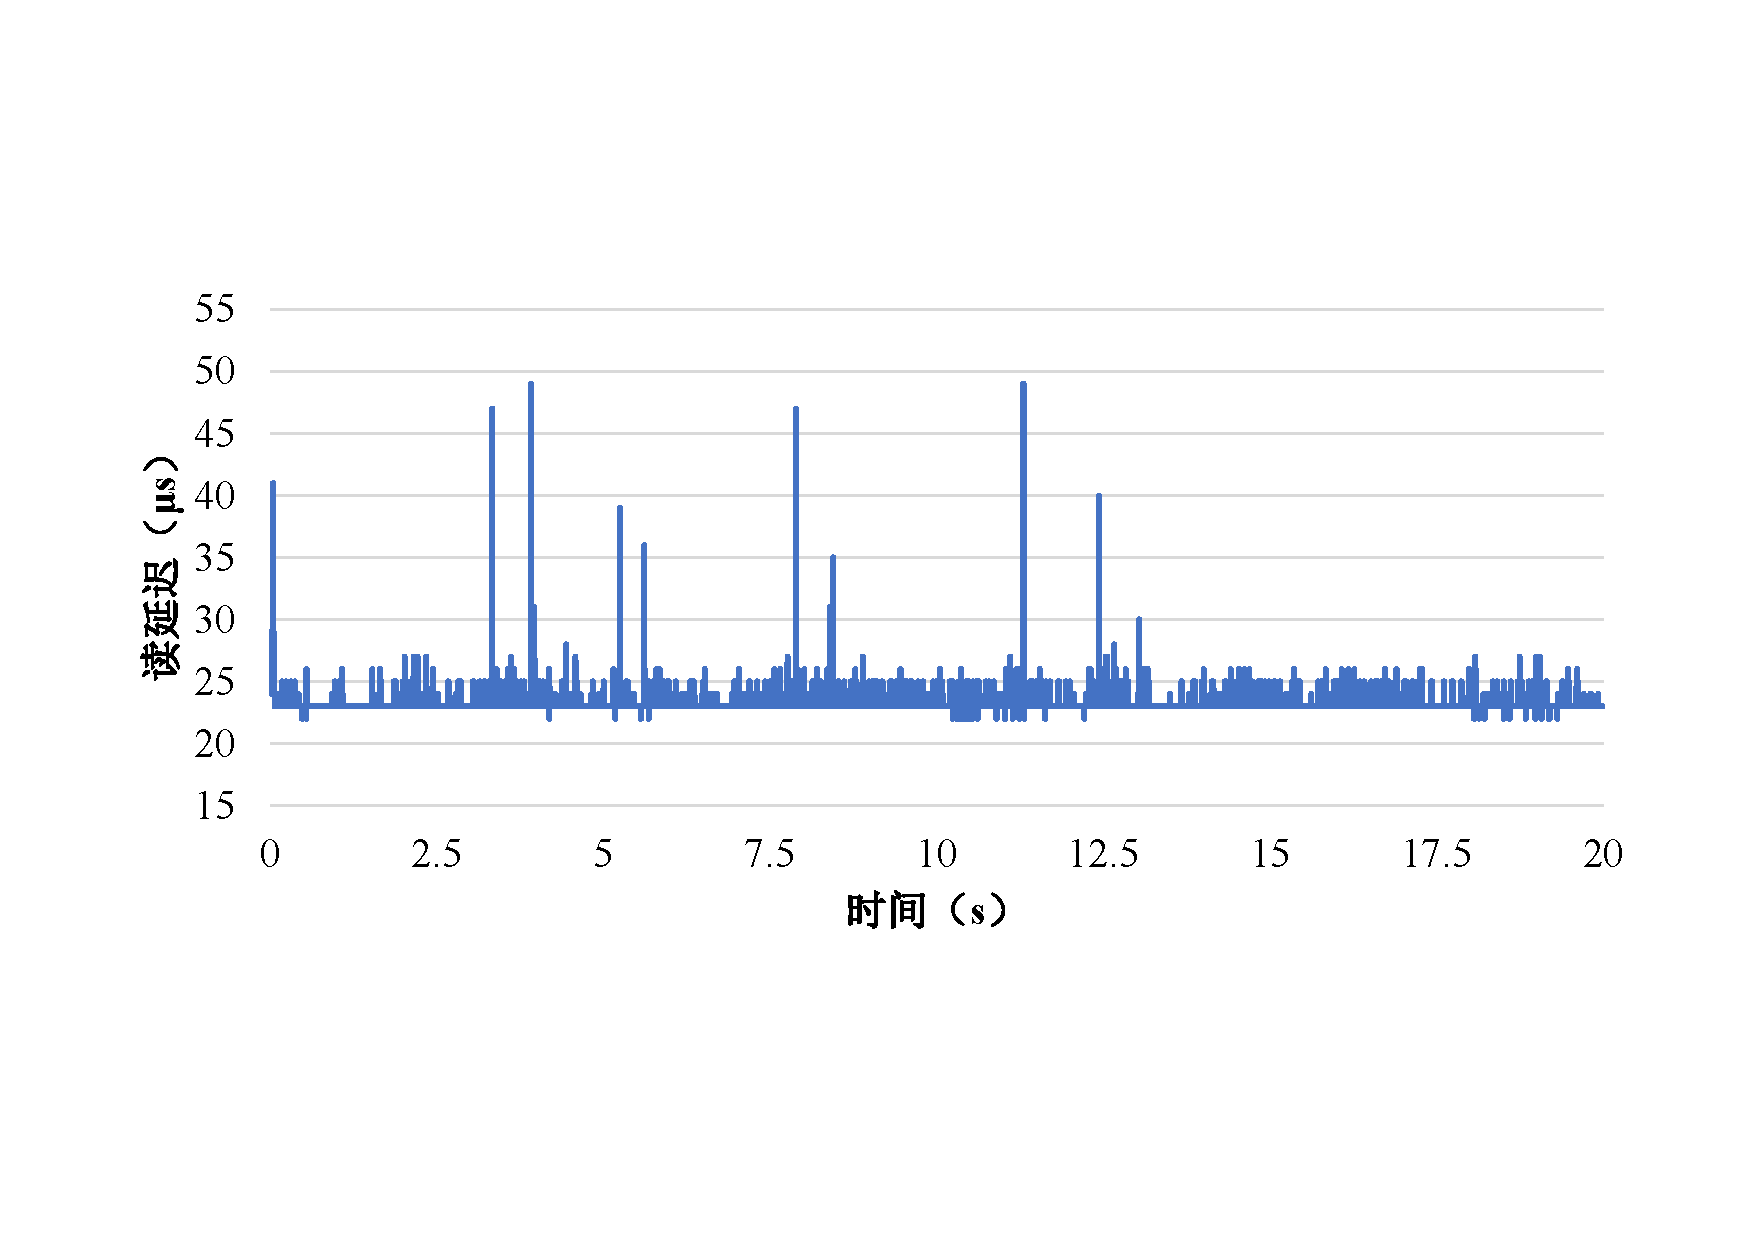
\includegraphics[width=13.5cm]{with-firstk.pdf}}   
    \caption{禁用和使用前-k 读取策略时的读操作延迟曲线}
    \label{fig:first_k}
\end{figure}

在不使用该策略时,读延迟平均值为 $\SI{22.38}{\us}$,读延迟曲线产生了明显抖动,有大量的读操延迟了 $\SI{30}{\us}$。使用该策略时,读延迟平均值为 $\SI{22.16}{\us}$,延迟曲线虽然仍然出现了一定的抖动,但少有延迟超过 $\SI{30}{\us}$ 的情况发生,读性能的不稳定性明显较小。可见,在 RDMA 网络环境下,前-k 读取策略虽然不能明显降低读操作延迟,但能明显使性能表现更加稳定。
